\documentclass{IEEEtran}
\usepackage[utf8]{inputenc}
\usepackage{graphicx}
\usepackage{subcaption}
\usepackage{url}
\usepackage{amsmath}
\usepackage{wrapfig, framed, caption}
\usepackage{hyperref}
\hypersetup{
    colorlinks=true,
    linkcolor=blue,
    filecolor=blue,
    urlcolor=blue,
    citecolor=blue,
    pdfpagemode=FullScreen,
    }
\usepackage{tabularx}
\usepackage{tabularray}
\usepackage[hmargin=1cm]{geometry}
\usepackage{multirow}
\usepackage{verbatimbox}
\usepackage{float}
\hypersetup{breaklinks=true}

%Dissertation Checklist

%Your document must not exceed 12 pages of text, excluding figures, tables, references and appendices.
%This is subject to the usual policy on word and page limits available on LearningSpace.


%Useful links
% Checklist video
    %https://web.microsoftstream.com/video/e31c5307-aa21-4d75-a7fd-0eba425ae73b?referrer=https:%2F%2Flearningspace.falmouth.ac.uk%2F
%G-Power downloads
    %https://www.psychologie.hhu.de/arbeitsgruppen/allgemeine-psychologie-und-arbeitspsychologie/gpower
    %https://learningspace.falmouth.ac.uk/mod/resource/view.php?id=245797

\title{Evaluating the use of Adaptive Agents to Build Player-Companion Collaboration} 
%Evaluating Collaboration With AI NPCs to Build Player-Companion Relationships
%\title{To what extent does the use of adaptive agents help to build player-companion collaboration?}
\author{Andrew J. Scott}  
\date{September 2022}

\begin{document}
	\maketitle
	\pagenumbering{arabic}

\begin{abstract}
This dissertation demonstrates the use of adaptive agents for companion characters that can work with players in a real-time action game. The research focuses on using adaptive behaviours to create a sense of collaboration with the player. Using these techniques aims to preserve the companion’s agency by making them independent while also working towards the same goal as the player. By studying adaptive AI techniques used in RTS games, this research aims to evaluate its use in a real-time action game by creating an agent that uses Agent Modelling to analyse the players’ actions and use these actions to plan how to better collaborate with their play style. A play-testing session compared how users rated it against another agent with the same behaviours but no adaptive decision-making processes. From the data collected, there was no perceivable difference between the user ratings for either agent in this study. This may be a result of the fast-paced nature of action games, making it difficult for players to focus on how the AI is helping them. Further research could present other AI techniques that make these behaviours noticeable in such games.
\end{abstract}

 \begin{IEEEkeywords}
Games, Artificial Intelligence, Planning, Agent Modelling.
\end{IEEEkeywords}

\section{Introduction}
\label{Intro}

%Introduce the area of investigation

This research aims to investigate the use of AI techniques to create an AI companion in an action game. In recent years, many commercial games focus on player-companion gameplay and dynamics, such as the recent \textit{God of War} sequels, \textit{The Last of Us} and \textit{Bioshock: Infinite}. The companions in these games are among the most appraised in commercial games for how well their characters are presented in these games.

%Elaborate of general context

However, these games are also high-budget games with large teams of writers, voice actors and animators that help to sell these companions as likeable characters through performance. This is a difficult task for smaller teams. Another avenue for creating liked characters is AI, which may be more suitable for smaller teams that lack the resources for great performances and allows the focus of the characterization to be in gameplay.

Specifically, this research investigates how to use AI techniques to build a sense of teamwork and collaboration between the player and their companion in an attempt to make the companion character likeable. Additionally, the companion presented in this research aims to be able to maintain their agency to be viewed as a character rather than just a companion. As such, the resulting companion cannot be explicitly commanded or controlled by the player and acts of their own accord.

This research produces a framework for a companion agent that can be used on its own or combined with writing, voice acting and high-quality animations to create a companion character. The techniques applied to this agent allow it to collaborate with the player by responding to their actions, but it cannot be explicitly commanded so they maintain its agency. This framework is designed to be as generic as possible so that it can be scaled up with additional mechanics that can further enhance the companion but does not require specific behaviours to be collaborative.

%Narrow down into specific topics

To do this, this research looks at AI techniques used in commercial games and academic research with a focus on building a team-working dynamic between a player and an agent. Most techniques that focus on this are in strategy games, which are generally slower in pace compared to action games. This research evaluates these techniques and looks at adapting them to work for a companion in a fast-paced action game.

In the next section, this dissertation summarizes the motivations for the project. In section \ref{RelatedWork}, this dissertation analyses design practices and AI techniques and how these can be used for this companion agent. Section \ref{ProposedResearch} details the research questions and hypotheses that will be tested. Section \ref{Artefact} demonstrates the AI technique used, the development of the artefact and quality assurance. Section \ref{ResearchMethod} details the design of the experiment, how the data is collected and the ethical considerations of the project. The data collected from the play-testing session is analysed in section \ref{Results} and the performance of the agents is evaluated in section \ref{Discussion}.

\section{Background}
\label{Background}

%TODO mid - restructure background and related work
%Background should illutrate important concepts and terminology to the reader, whilst the related work section should critique the existing literature in your area of study. 

A key motivation for this work is a developer conference by Constantine et al. that focused on building the relationship between the players and their ally, Aurene, so that their death feels more meaningful \cite{EGXCharacterDeathGuildWars}. One of their points was that allowing players to be explicitly command companions can ruin their agency.

When developing the AI for \textit{Atreus} in \textit{God of War}, there was a lot more of a focus on the sense of teamwork between Atreus and the player \cite{GDCAtreus}. This can be overshadowed as the player can explicitly command Atreus, which can ruin his agency \cite{EGXCharacterDeathGuildWars}. This research intends to create an AI that can collaborate with a player like Atreus but is independent like Aurene.

This research builds upon combat AI for companion characters by focusing on the sense of collaboration between them and the player while maintaining this independence. Collaboration in this research is defined as the sense of teamwork between the player and a companion NPC. This is built with synergistic behaviours where the AI makes it easier for the player to play the game noticeably. To do this, this research presents an adaptive agent, which changes its behaviours in response to the player's actions. The intention is that responding to the player's actions will make them more collaborative.

The agent will have to balance multiple duties, such as helping the player stay safe, attacking other enemies so they do not get overwhelmed and maintaining its safety \cite{CoupledEmpowermentMaximisation, tremblay2013adaptive}. To preserve player agency, the AI should not overshadow the player and will use mostly supportive behaviours to assist them \cite{DesignDocAIAllies}.

The combat actions for both the player and companion will be simple. This reduces the scope and allows the AI to be incorporated into other action games easier. This is standard AI practice in the industry, and many Game Developer Conferences (GDC) talk about simplifying AI behaviours \cite{GDCLessIsMore, GDCSimplestAITrick}. While the player should be able to notice the AI, they should not need to rely on them for specific behaviours or completely change their play style to get the AI to be helpful.

\section{Related Work}
\label{RelatedWork}

Research in 2010 highlights the lack of AI research in games \cite{RealTimeAICritique2010}. Since then, there have been a lot of improvements in AI research. Specifically looking at companion characters, there is a lot of research on implementing adaptive behaviour.

Friedman and Schrum analysed two companion bots in a first-person shooter \cite{CompanionBotsFPS2019}. The ratings for the helpfulness of the companions were similar, which they said may have been due to vague terms. Adaptive agents that focus on being effective were rated as helpful due to the points they scored and their ability to survive better than non-adaptive agents. However, the non-adaptive agents that stayed near the player were also scored as helpful because they were seen in gameplay often. Players that rated the non-adaptive agents as more helpful justified this as they felt a stronger sense of teamwork and the game experience mattered more to them than points.

Geib et al. present a plan recognition approach that allows an agent to analyse the actions of another and use those actions to determine what plan is being attempted \cite{GeneratingCollabBehaviourPlanRecognition2016}. Unlike the agent by Friedman and Shrum \cite{CompanionBotsFPS2019}, this AI uses adaptive techniques to collaborate with another agent. This plan recognition agent adapts to the actions taken by another agent to determine their plan. Once a plan has been determined, the agent can work through the already completed steps to determine what still needs to be done and takes actions towards these steps.

One of the more novel approaches, demonstrated by Tremblay and Verbugge, was to have a companion AI that can analyse the game intensity and change its behaviour as a way to dynamically adjust game difficulty \cite{tremblay2013adaptive}. Though this is not an example of AI adapting to another agent's actions, it still demonstrates the effect adaptability can have on the user experience.

In industry, games like \textit{God of War 2018}, \textit{The Last of Us} and \textit{Bioshock Infinite} are renowned for their AI companions \cite{PlayDontShow}. All three of the studios behind these games have developed AI techniques to fine-tune behaviour.

\subsection{Responsive Behaviour}
\label{Responsive Behaviour}

Atreus in \textit{God of War 2018} is a good example of synergistic AI, as he will help the player land slow attacks and will extend enemy vulnerability by shooting them with arrows \cite{GDCAtreus}. For example, when the player launches an enemy into the air, Atreus will shoot them and keep them there.

There is also an emphasis on his character development throughout the game, which is reflected in his behaviour. At the start of the game, he only takes actions when commanded, and learns to be more automated towards the middle of the game. Later, he becomes brash, so he starts to outright ignore the players’ commands and performs actions that would otherwise only occur when commanded like his special runic abilities.

These changes in his AI help to tie the narrative into the gameplay and make him seem like a real character, which helps to allow the player to bond with Atreus. These changes are also noticeable when the player is separated from Atreus, which helps the players realise how much they rely on him.

% TOTO - Include other sources that talk about responsive behaviours

\subsection{AI Movement}
\label{Movement}

%Image of pathfinding with caption
\begin{figure}
  \centering
  \includegraphics[width=\linewidth]{Images/IndustryResearch/TLOUPathfinding.png}
  
\caption{Pathfinding diagram in \textit{The Last of Us}}
\label{fig:TLOUPathfinding}
\end{figure}

Pathfinding is an important aspect of AI companions. The AI needs to be close to the player so that it is not forgotten \cite{GAIP2EllieAI}, but also not too close that it gets in their way and obstructs them \cite{CoupledEmpowermentMaximisation}. An example of poor AI pathfinding is in \textit{Skyrim} \cite{tremblay2013adaptive}, where the AI will move in front of the player when they are aiming and generally get in their way when moving. Naughty Dog addressed issues like this in \textit{The Last of Us} with pathfinding tools, shown in figure \ref{fig:TLOUPathfinding}, that keeps companions close to the player, but not in the way \cite{GAIP2EllieAI}. Ellie will also move out of the way if the player moves into her personal space. Vocal barks are used in such moments to add character, and it is a good practice to use voice acting to help make the player aware of the agent’s actions and make them feel more real \cite{GMTGoodAI}. However, they may not be suitable for games with lower budgets.

%Images of fight circles with captions
\begin{figure}
  \centering
  
  \begin{subfigure}[a]{\linewidth}
  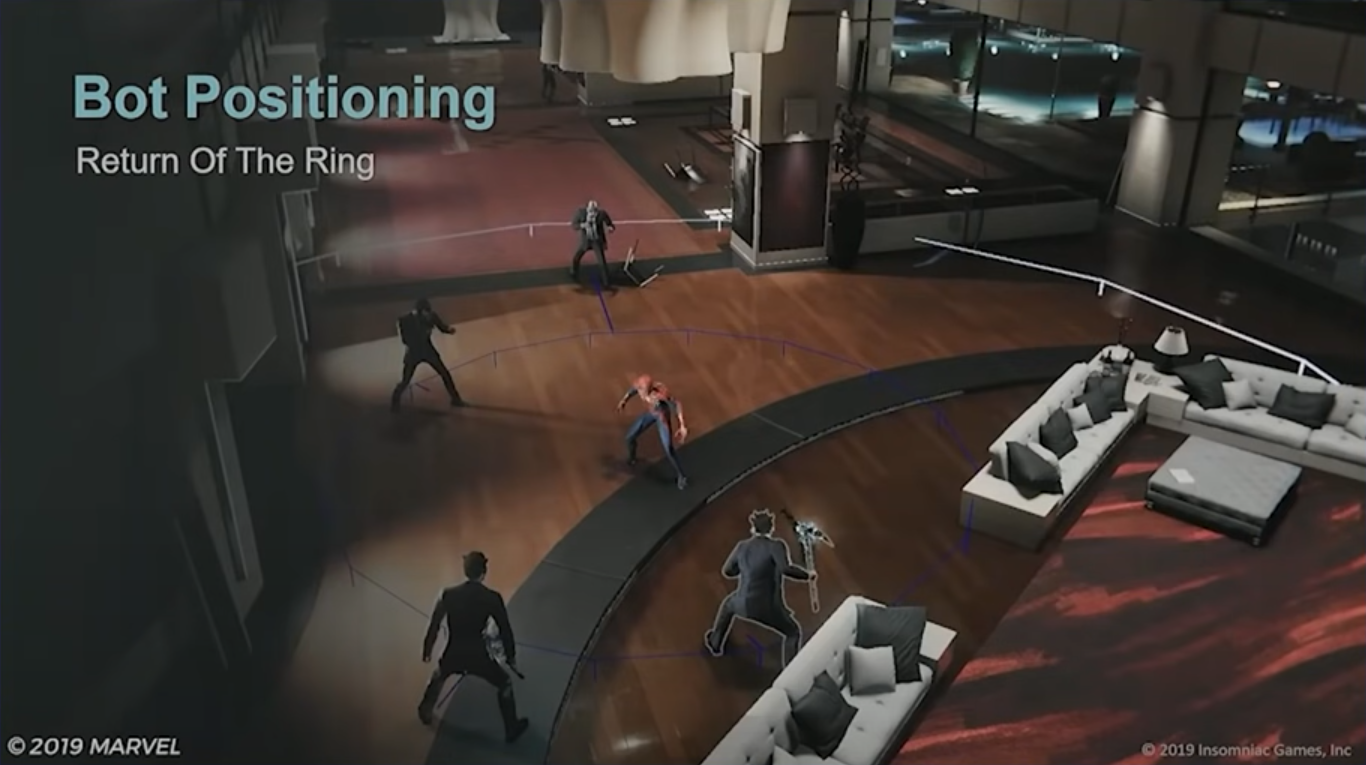
\includegraphics[width=\linewidth]{Images/IndustryResearch/SpidermanKungFuCircle.png}
  \end{subfigure}
  
  \begin{subfigure}[b]{\linewidth}
  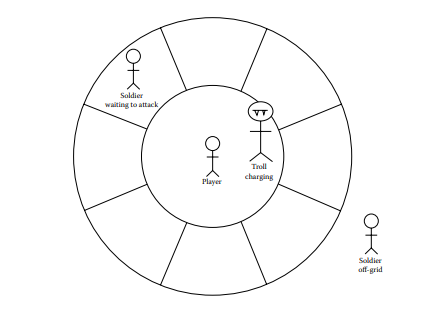
\includegraphics[width=\linewidth]{Images/IndustryResearch/KOARKungFuCircle.png}
  \end{subfigure}
  
  \caption{Demonstration of Kung-Fu Circles in (a) \textit{Marvel's Spiderman} and (b) \textit{Kingdoms of Amalur: Reckoning}}
  \label{fig:KungFuCircle}
\end{figure}

Many action games, such as \textit{Marvel's Spiderman} and \textit{Kingdoms of Amalur: Reckoning}, use a technique known as the Kung-Fu Circle to manage the positioning of multiple agents \cite{GAIPKungFuCircle, GDCSpiderman}, shown in figure \ref{fig:KungFuCircle}. An AI manager handles the positioning of enemies in this circle and manages when they can attack. While this technique is intended to manage multiple enemies in action games, it can be used to determine where the AI companion could be placed.

\subsection{Animations, Bespoke Behaviours and Call-outs}
\label{ABC}

A lot of industry practice with developing AI for companion characters is to use bespoke behaviour, detailed animations and vocal call-outs to give personality and character \cite{GMTGoodAI, GAIPOReactions}. These help to both characterise them and give player information \cite{GAIP2EllieAI}. In particular, Irrational Games created a smart terrain system for \textit{Bioshock: Infinite} that allows \textit{Elizabeth} to interact with the environment \cite{GDCElizabeth, AIGamesBioshockAI}, shown in figure \ref{fig:BioshockSmartTerrain}. A lot of these finishing touches are a key part of making the companion feel more believable, allowing a player to empathise and engage with them more. It also helps to communicate NPC actions, so it is clear to players that they are making choices, otherwise, they can miss the intelligence of the AI \cite{GMTGoodAI}.

Instead of focusing on animation and voice lines, the agent presented in this research will use adaptive behaviours to improve the sense of collaboration between them and the players. The intent of this would be to improve player-companion relationships in games with lower budgets and to maximise them in games that can have animations and voice acting. To do this, it will feature AI techniques that allow a companion NPC to adapt to player actions to collaborate with them better.

\begin{figure}
  \centering
  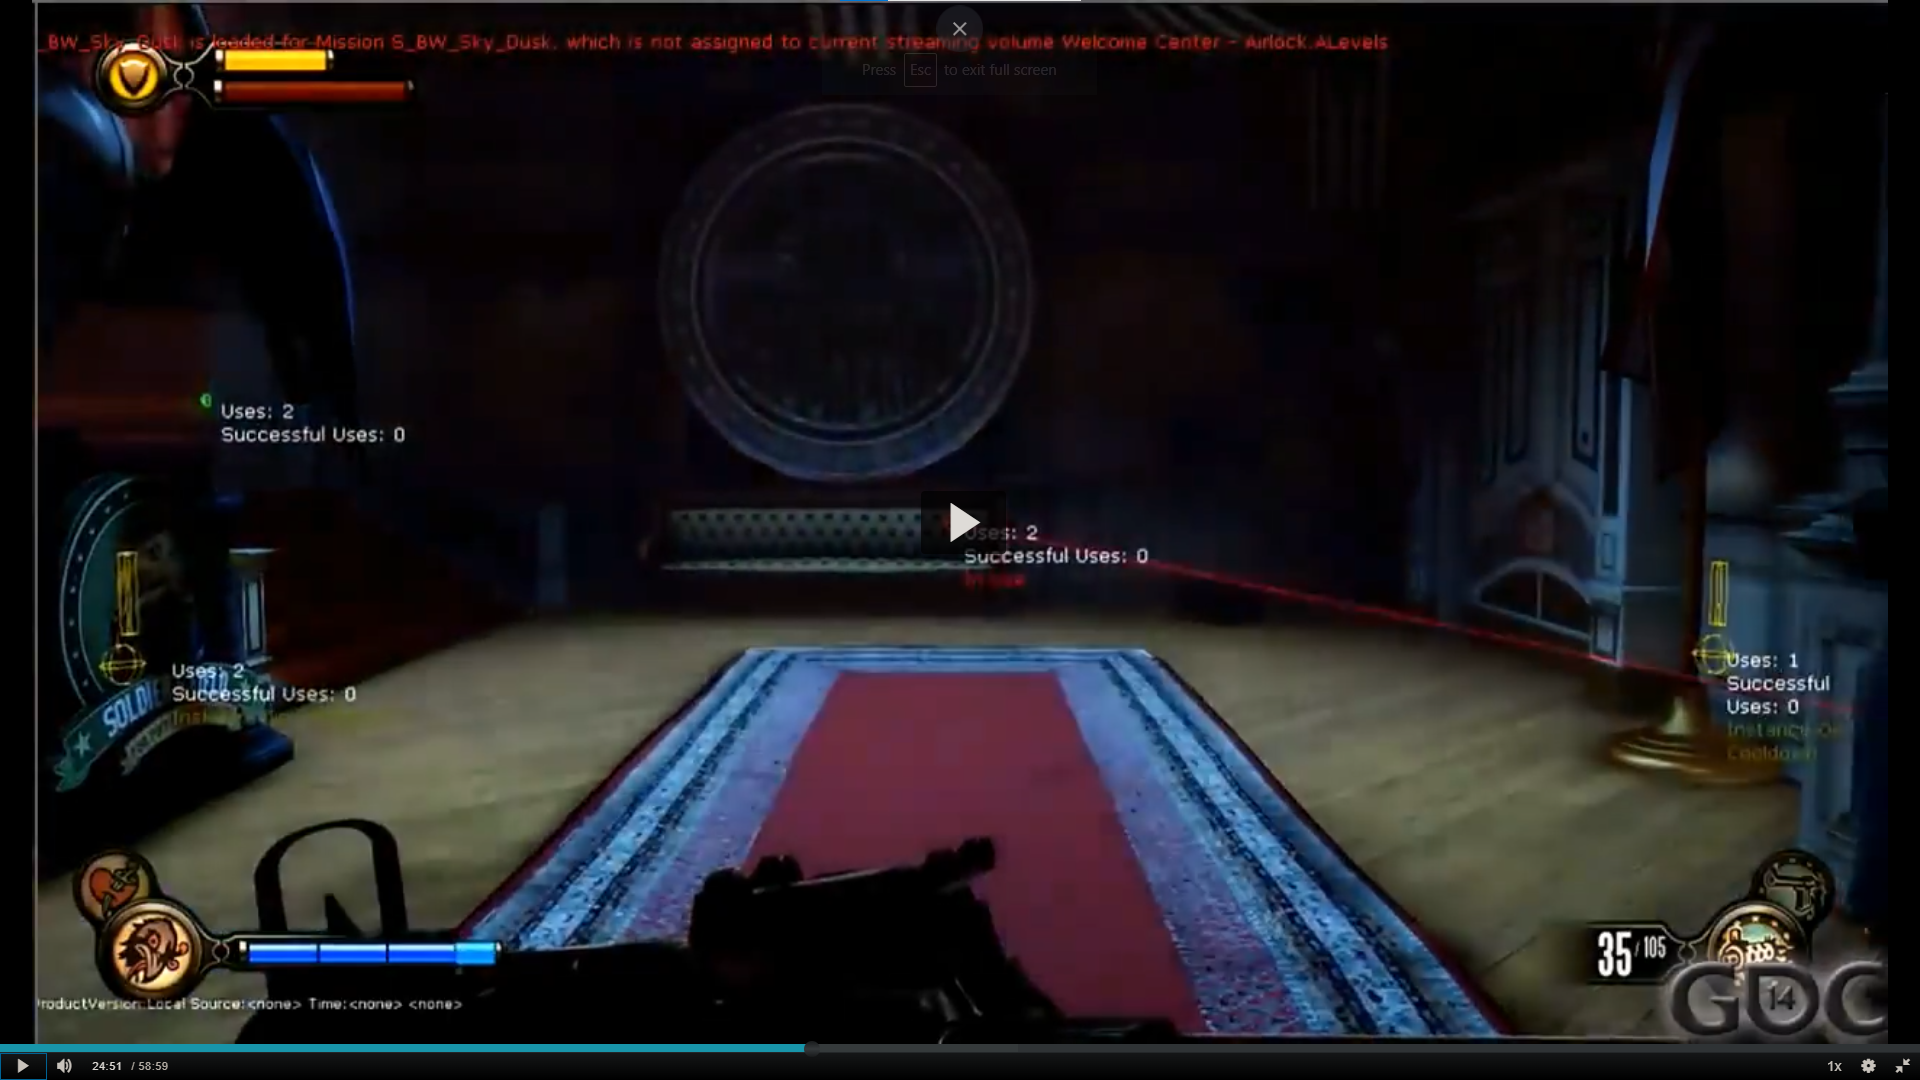
\includegraphics[width=\linewidth]{Images/IndustryResearch/BioshockSmartTerrain.png}
  
\caption{Smart Terrain showcase in \textit{Bioshock: Infinite}}
\label{fig:BioshockSmartTerrain}
\end{figure}

\subsection{Collaboration Without Communication}
\label{Communication}

\begin{table*}[ht]\centering
\begin{tabular}{ |p{0.5cm}|p{6cm}|p{6cm}|p{5cm}|  }
 \hline
 \multicolumn{4}{|c|}{Hypothesis Table} \\
 \hline
 Label & Hypothesis & Null Hypothesis & Test\\
 \hline
    H1 & The AM companion will be seen as more collaborative compared to the IT companion & 
    Using adaptive behaviours has no effect on how collaborative the companions are rated &
    T-Test between the collaboration ratings of both agent types \\
 \hline
    H2 & Players' user experience will be improved if they felt a greater sense of collaboration & 
    Collaboration has no effect on user experience &
    Correlation test between the user experience and collaboration ratings\\
 \hline
\end{tabular}
\caption{Hypothesis Table}
\label{HTable}
\end{table*}

The core design is that players cannot explicitly command the companion. As a result, the AI needs to determine how to collaborate with players without communication. The following methods are some ways in which an AI can collaborate with other agents without communication.

Board games like \textit{Hanabi} and \textit{Pandemic} are often used in academic research for collaborative AI as they involve teamwork between multiple players that cannot communicate with each other. Eger and Grus demonstrate a technique for \textit{Hanabi} that uses timing to communicate between agents \cite{WaitASecond2019}. While this is effective for collaboration between AI agents, this method is not reliable for player-AI collaboration as a human player isn't going to perform actions with specific timing to communicate with an AI agent.

Walton-Rivers et al. present an AI for \textit{Hanabi} that uses agent modelling to collaborate with other AI players \cite{EvaluatingHanabiAgents}. Agent modelling techniques involve observing actions taken by a player or another agent and using these actions to construct a model of them. This model describes how the observed entity acts and can be used by the AI to determine its actions. Yannakakis et al. demonstrate the use of machine learning to determine how an agent can use a player model \cite{yannakakis2013playermodelling}.

Agent modelling can also be used in Real-Time Strategy (RTS) games. Schadd et al. demonstrate the use of agent modelling for \textit{Spring} \cite{OpponentModellingRTS2007}. Bakkes et al. then build upon this research to use it in Case-based game AI \cite{bakkes2009opponentmodelling}.

%\cite{van2005opponent} - This tends to not be used for commercial games however (though this source is from 2005 so it may be out of date)

Plan recognition is another common technique that is used in board games. This is another technique for agents that need to collaborate with other agents, including players, without requiring explicit commands or communication. Agents that use plan recognition observe the actions, similar to agent modelling. However, instead of constructing a model of a player, it identifies the player's goals by comparing the steps required to achieve that goal to the steps that have been taken \cite{GeneratingCollabBehaviourPlanRecognition2016}. Once an entity’s goal has been identified, the plan recognition agent will devise actions that can aid them in achieving their goals. The unfinished steps in the plan can be used as potential behaviours.

Sauma-Chacón and Eger evaluate plan recognition agents that can play with a human player in \textit{Pandemic} \cite{PandemicPlanRecognition2021}. This AI was able to play at a level similar to that seen in full teams of AI and was perceived as more helpful. In addition, they detected a correlation between perceived helpfulness and skill.

Like agent modelling, this technique can also be used in RTS games as agents use observed behaviour to determine their allies' or opponents' plans. Jansen uses plan recognition for an allied agent in RTS games, instead of as opponents \cite{PlayerAdaptiveRTSAI2007}. This agent can look at players' actions and build units to support their plans.

\section{Proposed Research}
\label{ProposedResearch}

\subsection{Research Question \& Hypotheses}
\label{Hypotheses}

%Todo Mid - In the final dissertation, re-articulate hypotheses in forms that align with null-hypothesis significance testing
%TODO mid - hypothesis table formatting

The use of adaptive behaviours in companions can affect various aspects of the gameplay. As shown in table \ref{HTable}, two hypotheses will test these effects. The main aspect this research tests for is creating a sense of collaboration between a player and companion agent during combat and the question this research attempts to answer is \textit{To what extent does the use of adaptive agents help to build player-companion collaboration?}

This question is the focus of the first hypothesis; The Agent Modelling (AM) companion will be seen as more collaborative compared to the Interval Timing (IT) companion. This will be tested in the experiment detailed in section \ref{ExperimentalDesign}. Comparing the rankings for the collaboration of both agent types using a T-test will determine if the behaviours result in a greater sense of collaboration.

The null hypothesis here is that adaptability has no discernible effect on the players' perceptions of collaboration or that it is rated as less collaborative. This will be determined if there is no significant correlation, or a negative correlation, between the agent type and the rankings for collaboration.

The second hypothesis is that there will be a correlation between the rankings for the participants’ sense of collaboration and user experience. In an experiment by Friedman and Schrum, some players rated the non-adaptive agent as more helpful because it was seen more in game-play, even if it scored lower in the game \cite{CompanionBotsFPS2019}. Players justified this as it gave them a better player experience and a sense of teamwork. A correlation test between the user experience and collaboration ratings is used to test this.

\section{Artefact}
\label{Artefact}

\subsection{Artefact Details}
\label{ArtefactDetails}

This research presents an adaptive agent for an action game that responds to a player's actions to collaborate with them\footnote{Github Repository:

\url{https://github.falmouth.ac.uk/Games-Academy-Student-Work-22-23/Buddy-NPC-Dissertation}}. This agent will be referred to as the AM agent. The intention is that this collaboration will improve the player experience, and this is one of the factors that is tested. UML diagrams of the adaptive agent can be found in appendix \ref{AppendixUML}.

The AM agent has general path-finding behaviours that keep it close to players or enemy targets and it will try to stay within the player's vision so they notice it. The AI features a behaviour tree to determine its tasks. the tasks mostly involve staying near the player and attacking nearby enemies.

This agent features agent modelling, detailed in \ref{Communication}. When the player performs a combat action, the AM agent will be given information about what kind of action the player took and whether they were successful. It uses this information to construct a model that describes how the player acts. This model is made up of key descriptors that describe the player's actions.

Every time the player takes aggressive actions, such as attacking, the AM agent will add to an aggressive descriptor. However, if they miss, it will add to a panic descriptor. Each action will add to a specific descriptor and the amount they add will be tweaked in play-testing, see appendix \ref{AppendixQAPlan}. It will then use this player model in the behaviour tree when deciding what it will do.

For example, if the player is aggressive, but is getting hit a lot, the companion AI may use flanking behaviours to attempt to draw enemies away from the player so they can focus on fewer targets. However, if the player is very defensive, and tends to attack only after enemies attack, the adaptive agent may focus on the player's current target and create an opening for them to attack. If the player is getting overwhelmed by enemies, the agent may try to draw enemies away from the player to give them some space to relax or it will intercept itself between the player and their enemies. UML diagrams are in appendix \ref{AppendixUML}.

A plan recognition approach would have required the player to think about their strategy more, which would suit a slower or more strategic game. An action game is fast-paced and because the player does not have as much time to think, they won't be able to come up with plans. As a result, this project will feature a player modelling approach because it can work better with a simpler combat system but still enables adaptive behaviour.

\subsection{System Development Life-cycle}
\label{DevLifecycle}

The project follows a waterfall methodology. A task board was used to break down features into smaller tasks and track the progress of the development and version control was used to track changes. This task board can be found in appendix \ref{AppendixTrelloBoard}.

The initial prototype\footnote{Github Repository (Initial Prototype):

\url{https://github.falmouth.ac.uk/Games-Academy-Student-Work-22-23/Buddy-NPC-Dissertation/commit/493e0063025132e950696b4d174af48a5b190060}} features a basic combat system. The player can move, attack, parry and dodge and these basic mechanics were not changed much in later commits. The agents in this commit use the update loop instead of a behaviour tree and chase their closest enemy and attack when they are in range.

The agent modelling is in a prototype state in this commit and does not affect the agents' actions. The agent modelling script can observe actions performed by a specified character and assign a basic descriptor that defines their dominant play style.

Subsequent commits\footnote{Github Repository (First Refactor):

\url{https://github.falmouth.ac.uk/Games-Academy-Student-Work-22-23/Buddy-NPC-Dissertation/commit/ff3c28e4a07d2bb3549c6dbc93962801a3e29a72}} implemented a behaviour tree, which allows for easier modification and extension to the AI. The AI agents were also being designed. Commits after this point are labelled “feat: Basic AI”, “feat: Adaptive AI”, “feat: Interval AI” or “feat: General AI” to show which agent was being developed. Updates to the AM agent were made in "feat: Adaptive AI" commits.

Some of the key mechanics and changes that emerged from the development included flanking and intercepting behaviour. The original plan was to have the AM agent flank when the player is performing counterattacks against their enemies. However, this did not produce much of a difference compared to normal movement, since it would usually move behind the enemy anyway.

However, it did produce behaviour that resulted in it drawing enemies away from the player, which was more suited to if the player was struggling so this behaviour was moved to the panicking model instead of the counter model. Now, when the player is dodging a lot, the AM agent will rush to the player and attempt to draw enemies away from them so they can focus on parrying attacks or countering.

\subsection{Validation and Verification}
\label{Validation}

The original quality assurance plan can be found in appendix \ref{AppendixQAPlan}.

\subsubsection{Unit Testing}

Unit tests were derived for certain calculations to ensure that they were correct. Most commits tagged “chore: Maintainability” implement unit tests. the figures in appendix \ref{AppendixUnitTests} show these tests.

The first set of unit tests contains edit mode tests that assert the flank position helper function. It passes a series of vectors through the function and confirms that they are almost equal (threshold = 0.1) to the expected value. When designing these unit tests, it was discovered that passing in a negative value for the distance would return a position between the targets. From this, the idea for a new behaviour emerged where the agent will position itself between the player and their enemies to help protect them.

Most of the unit tests were for play mode. The first set of play mode unit tests was designed to test the model generator script. These tests assert that taking actions will generate the correct player model and it does so independently of the combat scripts, so it only checks the model script.

Expanding on this, unit tests for the combat script were developed. These tests extend these checks by determining that the model is generated correctly from actions within the combat script. These tests found an issue with the attack, dodge and parry actions, which would cause the model to think the player is panicking. These occurred from a function within these actions where they would end the current attack, which causes the model to think that the character made an attack. This issue was then fixed.

The final unit tests focus on the health scripts. These commits assert that the health is correctly calculated from damage taken and healing received. It also checks that the player should be killed if they receive damage that brings their health below 0. Additionally, the second commit contains a change that prevents healing above max health by clamping the health value.

\subsubsection{Integration Testing}

During the development of the artefact, incremental integration testing was used to ensure individual elements were implemented properly.

The initial prototype focused on the player mechanics and the character animations. The AI implemented in this prototype had some of the basic behaviour needed to test the combat mechanics. The AI for both the companion and enemies did not use a behaviour tree in this prototype, instead using the update function to determine actions.

The player model in the initial prototypes also had no influence on the companion's behaviour in this initial prototype, but it was implemented and the player state was displayed on the UI to test how player actions influenced it.

Various scenes within the project are used to test specific mechanics. For example, scenes where the health is set extremely high for all characters to focus on testing AI changes in combat, and a scene with just the player and an enemy is used to refine combat mechanics.

\subsubsection{System Testing}

These behaviours were tested with pilot play-testing with verbal feedback to ensure that the player model is constructed properly and that appropriate actions are taken based on the current player state. From this initial play-testing, players were struggling with the high difficulty as enemies would swarm the player and constantly attack them. This high difficulty was intended to force the player to rely on cooperating with their ally, but players found it too stressful to notice the AI.

The combat difficulty was reduced by making changes to the enemy AI to reduce swarming behaviours. A cooldown was added between attacks and adjustments were made to the enemy AI to move enemies away in a small circle if they cannot attack, similar to the Kung-Fu circle method originally used in \textit{Kingdoms of Amalur: Reckoning} \cite{GAIPKungFuCircle}. This reduced frustration and stress while allowing the player to notice their companion more.

In addition, various quality-of-life changes were made to the camera, UI, inputs and attack animations to make the game more intuitive and accessible.

\section{Research Methods}
\label{ResearchMethod}

\subsection{Philosophical Position}
\label{PhilosophicalPosition}

%What is this thing called Science? https://falmouth.primo.exlibrisgroup.com/discovery/fulldisplay?context=L&vid=44FAL_INST:44FAL_VU1&search_scope=MyInst_and_CI&tab=Everything&docid=alma9911072374905136
%Scientific Method https://plato.stanford.edu/entries/scientific-method/
%Philosophy of Science https://undsci.berkeley.edu/the-philosophy-of-science/
%Philosophy and Paradigm of Scientific Research https://www.intechopen.com/chapters/58890 

%TODO Low - research empirical philosophy to see if it fits better
% TODO Low Justify philosophies

The research was carried out using positivist philosophies \cite{Zukauskas18}. A survey was used to collect quantitative data that analyses the effect of AI adaptability on the player's collaboration with the AI agent, and how that affects their opinions on the AI. There were some questions with qualitative answers, but these were used to assure that there are no issues with the study.

\subsection{Experimental Design}
\label{ExperimentalDesign}

%Might be best to have each participant play both as they could be skewed by personal biases so the baseline needs to be established randomise the order

%G-Power video explanation: https://web.microsoftstream.com/video/d1ec1c56-bb97-4592-ae4e-1c973e3fee20?referrer=https:%2F%2Flearningspace.falmouth.ac.uk%2F

The experiment took place on campus at the Games Academy Warehouse.

Players will be presented with a third-person action game. The player will play through a tutorial and two combat encounters, each with five opponents for them to defeat. Defeating all of the enemies will load the next level. In both combat encounters, the player will be accompanied by a different AI companion. The order in which they play with the AI companions is randomised to avoid observer bias \cite{hrobjartsson2013observer}. Once they have played through the demo, the participants were given a questionnaire form to fill out. The link to the questionnaire is in appendix \ref{AppendixLinks}.

The first companion is the AM companion described in section \ref{Artefact}, which uses player actions to calculate the state the player is in, and uses a behaviour tree to determine which actions to take based on this state. AM will determine targets based on the player's actions and choose behaviours that support their intentions better.

The original plan was to test the AM agent against the simple AI already implemented in the initial prototype, see section \ref{DevLifecycle} for more details. However, during development, it was decided that this would not be a fair experiment as the simple AI does not have access to the same behaviours. As such, the IT agent was developed to properly test the AM agent. The IT agent has access to the same behaviours, but instead of using the player state through the player actions, it randomly changes between states every three to eight seconds.

Most of the questions in the survey use a Likert scale and will include questions on how likeable, intelligent, collaborative, etc. the player thought they were, using a similar approach used by Z. Ashktorab et al. \cite{SocialPerceptions2020}. There will be some qualitative questions that allow participants to put sentence answers so they can give more specific thoughts. This will also help to determine if any bugs caused one AI to not work as intended.

% TODO Low: Cite likert scale central tendency

The questions will use a seven-point Likert scale. Using a seven-point scale gives more accuracy as it reduces a central tendency bias. This is caused when participants avoid choosing extreme responses to avoid seeming like they have extremist values.

\section{Ethical Considerations}
\label{EthicalConsiderations}

%TODO high - In the final dissertation, expand your ethical considerations. Cite key legislation (e.g., GDPR), international law (e.g., Declaration of Helsinki), and codes of conduct (e.g., Falmouth University Research Integrity Policy and BCS Code of Conduct).
% TODO high - Refer to the content of your application for ethical approval and any risk assessment (e.g., health and safety) you’ve conducted. Then, enrich your analysis with a more balanced insight into risks and benefits. Consider the potential wider benefits your work could pave the way for.

The data collection involved an experiment that focuses on various AI behaviours, and how different behaviours can build a stronger emotional connection between players and AI companion NPCs. As such, participants were involved. Participants tested the AI and filled out survey forms to give their opinions on the various AI mechanics. Under these criteria, there are no high-risk categories, but since participants are involved, it counted as a medium-risk experiment. The Nuremberg Code, the Falmouth University guidelines and the BCS Code of Conduct have been followed to protect the rights of the participants \cite{germany1949trials, BCSConductCode}.

The participants were given information forms that detail the experiment and their participation in it. This information sheet is in appendix \ref{AppendixEthicsForms}. There are no aspects of the experiment that are hidden from the participants, and the form has clear information on what the experiment will entail. The form has information on the purpose of the research, expected duration, procedures, what the participants are being asked to do, their right to decline and withdraw, confidentiality and contact info for the researcher.

To participate in the experiment, participants were asked to sign that they understand and agree with the form, no signature will be required as it is an online form. A screenshot of the consent form is also in appendix \ref{AppendixEthicsForms}. Participants will also be required to state that they are at least 18 years of age to participate in the experiment. However, they will not need to state their age, only that they are above 18 years old. There will also be no transactions or other coercion to participate in the experiment.

All participants will be given a right to withdraw at any time and this will also be made clear in the information and consent forms. The forms will have contact information for them and a reference number so that their responses can be removed without requiring them to give any personal information. They will also be able to use this number to check their responses, though they will not be able to change their responses once submitted to preserve pure data, they can only be removed.

%TODO high - in the final dissertation, please consider making direct reference to legislation pertaining to personal data. As you are collecting data from people, you need to refer to GDPR. Either illustrate how your data does not meet the definition of personal data or justify the means through which you will ethically and legally manage personal data in your study design.

%Find source for GDPR

Despite involving participants in the study, the research remains GDPR compliant as no personal data will be collected. When signing that they agree to participate, no signatures, names or emails will be collected. Only a few questions allow for qualitative answers and none of them requires the participant to divulge any personal information. Once the data has been analysed, it will be archived until the study is complete, after which all responses will be deleted.

A risk assessment, which can be found in appendix \ref{AppendixRiskAssessment}, has also been completed. This addresses some potential risks that could occur as a result of the experiment and how they can be mitigated. Additionally, a risk matrix has been made that analyses the likelihood of these occurring in relation to the severity.

\subsection{Data Management Plan}
\label{DataManagement}

%Data management and questionnaire

The responses to the questionnaire were converted to a CSV file, and stored on an online network drive. This data was analysed using R Studio, outputting various graphs that visualised the data for readers and statistical tests were conducted to assert the hypotheses, detailed in section \ref{Hypotheses}. The R-Code and the links to the questionnaire and the summary are in appendix \ref{AppendixLinks}

Using G-Power, a sample size of 59 is required for T-Tests with an effect size of 0.4. This effect size was chosen because it is a medium-large effect size, as defined by Cohen \cite{cohen1988statistical}. A small or medium effect size may not be noticed by most players, especially in a fast-paced action game, as they may be more focused on fighting their enemies.

%G-Power downloads
    %https://www.psychologie.hhu.de/arbeitsgruppen/allgemeine-psychologie-und-arbeitspsychologie/gpower
    %https://learningspace.falmouth.ac.uk/mod/resource/view.php?id=245797
    
\begin{table*}[t]\centering
\begin{tabular}{ |p{0.5cm}|p{6cm}|p{6cm}|p{5cm}|  }
 \hline
 \multicolumn{4}{|c|}{Hypothesis Table} \\
 \hline
 Label & Hypothesis & Null Hypothesis & Test\\
 \hline
    H1 & The AM companion will be seen as more collaborative compared to the IT companion & 
    Using adaptive behaviours has no effect on how collaborative the companions are rated &
    T-Test between the collaboration ratings of both agent types \\
 \hline
    H2 & Players' user experience will be improved if they felt a greater sense of collaboration & 
    Collaboration has no effect on user experience &
    Correlation test between the user experience and collaboration ratings\\
 \hline
    PH1 & Players will rate their agent as more collaborative if they thought they were more adaptive & 
    Adaptivity has no effect on collaboration &
    Correlation test between the adaptivity and collaboration ratings\\
 \hline
    PH2 & Players will rate their agent as more believable if they thought they were more intelligent & 
    Intelligence has no effect on believability &
    Correlation test between the believability and intelligence ratings\\
 \hline
\end{tabular}
\caption{Updated Hypothesis Table}
\label{PostHTable}
\end{table*}

\newpage

\section{Results}
\label{Results}

%TODO mid - format hypothesis table at bottom of THIS PAGE

After carrying out the play-testing sessions, there were 59 participants. Four of their survey responses had to be removed because their forms were filled out incorrectly. This left 55 valid responses, each of which had two data points. As shown in table \ref{PostHTable}, additional tests were carried out to test two post hoc hypotheses.

% Table info https://tex.stackexchange.com/questions/53384/creating-a-table-in-two-column-style-page

\subsection{Hypothesis 1 - The adaptive companion will be perceived as more collaborative than the non-adaptive companion}

This hypothesis evaluates the players’ perception of collaboration between both agent types. A t-test between the collaboration ratings of both agent types returns a p-value of 0.2889. This high value means that the null hypothesis may be true.

\begin{figure}[!h]
  \centering
  \includegraphics[width=0.9\linewidth]{Images/Graphs/H1CollabPairBar.pdf}
  
\caption{Pairwise comparison bar chart displaying the difference in user ratings for collaboration}
\label{fig:H1CollabPairBar}
\end{figure}

There is very little difference in the collaboration ratings for each agent type. Figure \ref{fig:H1CollabPairBar} shows a pairwise comparison demonstrating that most players did not perceive a difference between agent types. In this graph, the ratings for each player were subtracted to show the differences between their ratings for each companion. Most players rated each companion equally, resulting in a difference of 0.

Additional graphs can be found in appendix \ref{AppendixGraphs}, which demonstrate that there is no perceivable difference between the collaboration ratings for either agent type.

\subsection{Hypothesis 2 - Players' user experience will be improved if they felt a greater sense of collaboration}

%TODO high - reduce number of figures here, put more detail in these 3 hypotheses to spread the images out

This hypothesis evaluates the correlation between the collaboration ratings and how much players enjoyed playing with that agent. A correlation test between these ratings returns a p-value less than 0.05 and a correlation of 0.4790956. This low p-value indicates that the null hypothesis may be false. However, there is only a modest correlation between the sense of collaboration and user experience.

\begin{figure}[!h]
  \centering
  \includegraphics[width=0.9\linewidth]{Images/Graphs/H2CollabUXScatter.pdf}
  
\caption{Scatter plot displaying the correlation between collaboration and how much they enjoyed playing}
\label{fig:H2CollabUXScatter}
\end{figure}

Figure \ref{fig:H2CollabUXScatter} shows a scatter plot that demonstrates the user ratings for their sense of collaboration and how much they enjoyed playing. A colour scale has been added to this graph to show how many participants rated each combination. The yellow dot indicates that most of the participants rated both companions as six on both of these categories. This shows a weak correlation between the ratings, but as their sense of collaboration increases, their rating for how much they enjoyed playing slightly increases as well.

\subsection{Post-hoc Test 1 - Players will rate their agent as more collaborative if they thought they were more adaptive}

The first post hoc test was used to evaluate how effective the use of adaptive behaviour is at fostering a sense of collaboration. A correlation test between these ratings returns a p-value less than 0.05 and a correlation of 0.516152. This low p-value indicated the null hypothesis may be false, though there is only a modest correlation between the ratings for adaptivity and collaboration. This could indicate that if the player perceived the agents as adapting to their behaviour, then they also collaborate with the player better as well.

\begin{figure}[!h]
  \centering
  \includegraphics[width=0.9\linewidth]{Images/Graphs/PH1AdapCollabScatter.pdf}
  
\caption{Scatter plot displaying the correlation between adaptivity and collaboration}
\label{fig:PH1AdapCollabScatter}
\end{figure}

Figure \ref{fig:PH1AdapCollabScatter} shows a scatter plot that demonstrates the user ratings for adaptivity and collaboration. This shows a modest correlation between the ratings between adaptivity and collaboration.

\subsection{Post-hoc Test 2 - Players will rate their agent as more believable if they thought they were more intelligent}

\begin{figure}[!h]
  \centering
  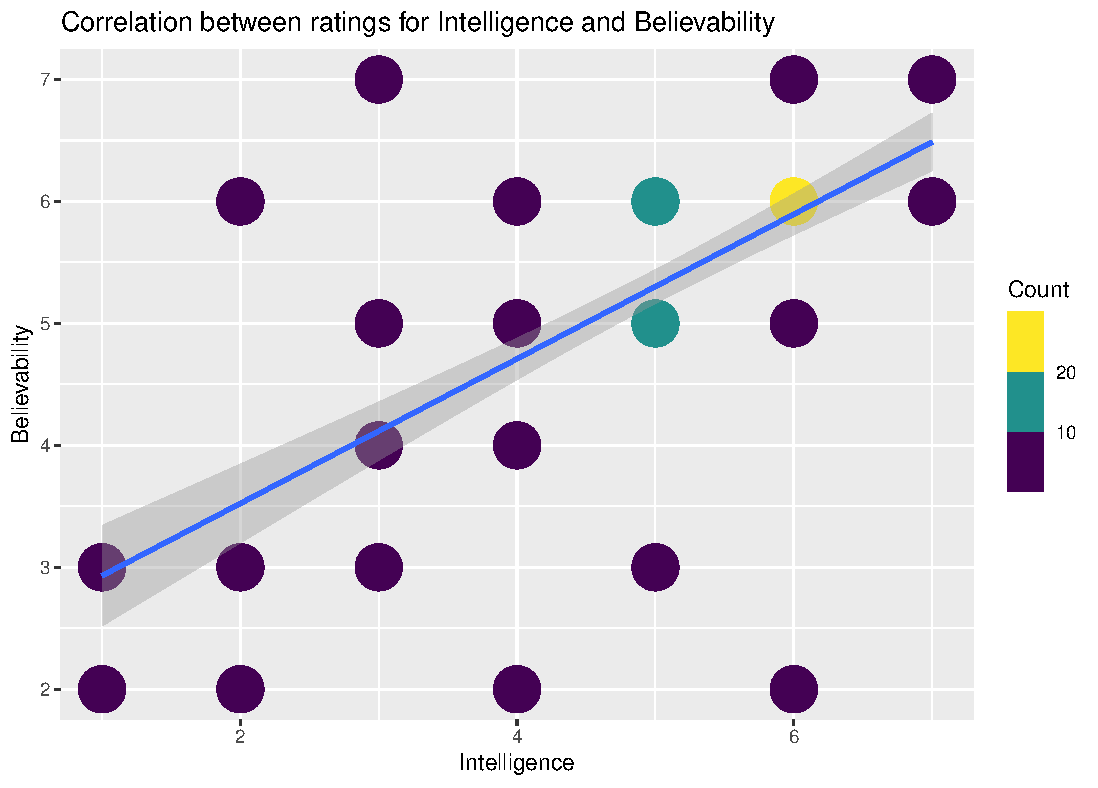
\includegraphics[width=0.9\linewidth]{Images/Graphs/PH2IntelBelieveScatter.pdf}
  
\caption{Scatter plot displaying the correlation between intelligence and believabilty}
\label{fig:PH2IntelBelieveScatter}
\end{figure}

This test was used to evaluate the effect perceived intelligence has on how believable the agents were. A correlation test between these ratings returns a p-value less than 0.05 and a correlation of 0.6011652.

There is a modest correlation between the ratings for intelligence and believability, which could indicate that increased intelligence ratings lead to the agents being perceived as more believable. The correlation value here is slightly higher than the others, though it is still modest.

Despite having the highest correlation value of the tests, a scatter plot for intelligence and believability ratings does not appear to show a strong correlation between intelligence and believability, as shown in figure \ref{fig:PH2IntelBelieveScatter}.

\section{Discussion}
\label{Discussion}

In this study, the use of adaptive agents alone was not enough to build a better sense of collaboration compared to agents with no adaptive behaviours. The results show near-identical perceptions between agent types. Pairwise comparisons were used to further examine any differences, and many responses indicate that there was no difference perceived between each agent type for all of the metrics the agents were measured on, including how adaptive and collaborative each agent was. This would suggest that the use of adaptive techniques alone is not enough to distinguish them from other agents. This could have been because the players were focused on fighting the enemies, and as such were unable to notice if and how their ally was helping them.

The changes in the companions’ behaviour are very subtle. Since one of the design goals was to make an AI agent that was generic enough to be used in various action games, all of the behaviours they perform are based on positioning (flanking, interposing or drawing enemies away). These provide only slight differences between the different AI states, which are barely noticeable to the player. One player also suggested that “(It) would be helpful if its actions were telegraphed somewhat, like through bark lines or colour indicators”. Using vocal barks would help distinguish similar behaviours as the AI could explain their actions or reasoning. This is a standard technique in industry, as shown in the AI for \textit{Ellie} \cite{GAIP2EllieAI}. Colour indicators or UI elements may not be as obvious in fast-paced action games but may be better suited for other types of games. Stealth games can use UI elements like sight-cones, awareness indicators and ghostly outlines to make the AI states obvious \cite{GMTStealthSenses1, GMTStealthDetection3}. Animations are also used to clearly show what state the AI is in \cite{GMTStealthDetection3}. These elements also help to make the AI more predictable as the player can clearly see they are following specific rules, which allows them to exploit their mechanics. Chris Hocking describes this as "The ability of the player to devise his own meaningful goals through his understanding of the game dynamics and to formulate meaningful plans to achieve them using the information and resources provided by the game" \cite{GDCIntentioalPlay}.

Additionally, the reasons the agents switch between these behaviour states are not obvious. Therefore, the players could have also perceived the random behaviour changes in the IT agent as adaptive behaviour, even if the agent was not adapting to player actions. When playing in a fast-paced action setting, the player may not be able to notice what behaviours the AI adapts to. Brown explains that good AI agents need to make the reasons for its behaviour obvious because the player does not know the agent's decision-making process \cite{GMTGoodAI}. The player has no way to know the agent is capable of making certain decisions if they do not make them obvious. One way of doing this would be having the companion give vocal barks, which help to both characterise them and make it clear what they are doing and why \cite{GAIP2EllieAI}.

The lack of time spent with each companion type could have also affected the players' perceptions. In such a short amount of time, the player may not be given the chance to learn how the AI responds to their actions. This could be better in a full game setting, where the player might be able to learn how the AI adapts and use this knowledge. Alternatively, the player would not be able to learn the IT companion because its random behaviours make it unpredictable. Chris Butcher, AI programmer for Bungie, stated "We don't do things by random chance very much. The goal is not to create something that is unpredictable. What you want is an artificial intelligence that is consistent so that the player can give it certain inputs." \cite{HowStuffWorksHaloAI}. While players perceived no difference between the agents in this research, it is possible that a longer play-testing session could give more time for the players to learn how the agents behave.

%TODO mid - One of the appraisals of Atreus' AI in the \textit{God of War} sequels is the bond between the characters and how it grows over the story. Part of this is how the player learns how to use him in combat

Looking at the qualitative feedback from the surveys, there were a lot of contrasting opinions on the behaviours like drawing enemies away or moving in between enemies and the player when they are struggling. Some players liked this kind of behaviour, remarking that “it felt like it had my back” for the AM companion and it “felt like it took more of the enemies away from me”. However, this was also intrusive for some players. One player stated that the IT companion “Kept swooping in to help me when I didn’t want it to”.

A lot of players had a greater mix of criticisms about the IT companion. Some stated that it was “Frustrating how quickly it changed enemies so often” or that it was “quite bad at properly focusing its attention on the right enemies”. However, others thought it was “more intelligent… as it was able to split the group of enemies up evenly” or it “adapted to my play style”. This mix of opinions could have been caused by the random behaviour changes, as it may have randomly chosen behaviours the players found helpful, or chosen behaviours at the wrong time and so felt intrusive. On the other hand, the feedback for the AM companion seems more consistent. Despite this qualitative feedback, the test results show no perceivable difference between the AI companions. This could indicate that the players did not notice the AM companion because there were fewer erratic behaviours. By not noticing the AM companion, they could have rated the companion with the same results.

Future-proofing is another consideration. Even though the IT agent was easier to implement, it would also be impossible to polish for a commercial product since the AI designer cannot make changes to the agent’s considerations, only the behaviours it can make. If the AI has access to special abilities, such as healing the player, it would not be possible for the IT companion to determine when to use them, since its actions are random. Alternatively, the AM agent can use the player state to determine when it would be the best time to use these abilities. In games with these types of actions, the AM companion may be preferred.

Some players felt overshadowed by their companions. Naughty Dog prevented \textit{Ellie} from dealing damage to enemies the player cannot see to address these issues while still making the AI seem active in the fight \cite{GAIP2EllieAI}. Since the agents only had access to melee attacks, this would have not been possible while also keeping the agent within sight of the player. However, maybe an idle state could be added to the player model, where the AI will try to move closer to the player to keep them more engaged in the fight if it notices that they are not participating in the fight.

Additionally, some players commented that they would like to be able to give commands to their companions. This would suggest that they felt the need for better control over the companion's behaviour. While this would give more control, commanding the agents may break the companion's agency as a character \cite{EGXCharacterDeathGuildWars}. This is also a game mechanic that may not suit every game.

While it seems that adaptive behaviours alone may not be enough to build a sense of collaboration, this research still presents an agent that can adapt to player actions. Combining this with other techniques may yield a more collaborative companion agent, or it could be used for creating enemies in games.

\subsection{Limitations}
\label{Limitations}

One of the key limitations was the choice to keep the AI agents generic by omitting to have special abilities or vocal barks for the companions. This choice was made to focus the research on the player modelling technique. Additionally, it enables a focus on providing a generic agent that can be scaled up to include these elements but does not rely on them.

However, these limitations made it difficult to design unique behaviours for various states that were noticeable since the only way to distinguish them was through positioning. In this research, the differences in the behaviours were too subtle for the players to notice and it was not clear why they were making specific choices.

The play time for the experiment should have been slightly longer. A small combat scenario may not have been enough for the players to notice any differences. However, in a longer session, the player may have the chance to discover the companions’ behaviour and learn how the agents respond to their strategies.

The experiment should have also been structured more intuitively. Instead of asking the participants to fill out the questions for both companions after playing with both of them, the questions should have been filled out for each companion one at a time. This would reduce the number of incorrectly filled questionnaires and remove any ambiguity that the participant filled in the questions for the wrong agent type. Additionally, the agents would be fresher in their minds when they fill out the questionnaire.

There were also a concerning number of participants who put that they agree (six) down for most of the questions. This could have been the result of a slight bias where the participants put down answers that they thought the researcher wanted them to. Including more negative questions like “I thought this companion was boring” could help filter such responses and make the participants think more about each question. Additionally, the questions could have been rated on a slider, which would also increase the range. The seven-point Likert scale was used because it allows the user multiple stages of agreeableness or disagreeableness, which helps to avoid a central tendency bias. Using a slider scale may reduce this as there is much more variety in how much the participant can agree or disagree with the statement.

Another limitation would be the number of responses. The target number of 59 participants was met, though four responses had to be removed due to incorrectly filled surveys, so the number of valid responses is slightly below the target.

% TODO mid - Consider threats to the validity of A|B tests. Mahoney's work on "Experimental Methods and Outcome Evaluation" would be useful to read to this end.
% Maybe AB testing with each player playing both sequentially was not useful as players that rated them noticed little difference. Maybe having each player play with 1 companion would have preserved more pure data

\subsection{Recommendations}
\label{Recommendations}

The agent modelling companion may perform better with more behaviours that have a greater contrast between them. While some of the positioning behaviours implemented are useful for cooperating with the player, this can be extended with special abilities that allow the companion to heal the player, or perhaps restore resources for them if they fit for the game. Many games, such as God of War or Bioshock, allow companions to use supportive abilities to cooperate better with the player, and this agent modelling approach could be used to determine when these actions would have the most effect on the player \cite{AIGamesBioshockAI, GDCAtreus}

Alternatively, there could be some feedback to let the player know what the companion’s actions are and why they are making them. An effective way to implement this would be with voice lines since the companion could explain why they are taking their actions, but some players suggested visual feedback like changing colours. This may not be as obvious for the player though as they would need to be able to see the companion, and having to look away from the action to find out what their companion is doing may be too distracting in a real-time action game. However, this may be preferable for silent games or those with smaller budgets.

More time could also be spent on refining the player model and behaviour trees. The feeling of being overshadowed by the companion could be reduced by tracking damage dealt or the number of kills by the player and companion and using those stats in the player model to determine whether the agent is being too active. If it is, then they could use more supportive behaviours.

Additionally, there could be more behaviours in each state to increase variety if the player’s play style is not changing much. There was a feature that allowed the agent to switch to the next highest states if they stayed in the same state for too long, though having greater variety within each state would be easier to polish.

The environment and gameplay design may also affect the agent. A more complicated combat environment with obstacles and cover could have provided more considerations for the AI. In addition, including a variety of enemy types would encourage the player to change their strategies, allowing the player modelling companion to change their play style to better reflect the new situation. The testing environment could have included a variety of combat scenarios with different enemy types and compositions, thus requiring the player to change their strategy. A similar method was used by Guckelsberger et al. when testing their CEM AI \cite{CoupledEmpowermentMaximisation}. Though this would be able to evaluate the agents more accurately, this would have been a little out of scope for this experiment to implement.

The difficulty is another consideration for how useful players found the AI. In the initial prototype, the game was designed to be difficult to require the player to use strategy and see value in their companion. However, verbal feedback from the quality assurance indicated that it was too frustrating and players were too busy to notice the companion, so the difficulty was reduced. Enemies were less aggressive and gave the player more breathing room, and the player had larger parry windows and they had a new action-cancelling mechanic. This allowed players to cancel any action with a parry or cancel dodges with attacks to make the controls more forgiving.

These changes may have made the game too easy, as the players did not have to think about strategy and button mashing became a viable strategy, which reduces how well the companion can adapt to the player. The easier difficulty also means that the players had more breathing room to notice and let the companion fight on its own, which is where some of them may have thought that it was overshadowing them.

A better balance in difficulty may have given the player the chance to notice the companion and not get frustrated, while also requiring the need for strategy. Additionally, a game with slower pacing would also make for a better environment for the AM companion since the player gets more of a chance to notice their companion’s actions. Further research could be conducted to determine the effects of difficulty on the player’s perception of their companions.

Additional variety and complexity in the enemies and environment would also give more opportunity for the agent to adapt. A well-designed cast of enemies can make the player change their strategy to fight them easier, and this would also allow their companion agent the opportunity to adapt to the player. Different combat scenarios with unique enemy compositions may make the adaptive behaviours more obvious to the player.

\section{Conclusions}
\label{Conclusions}

The results of the experiment show that the player modelling approach used has no perceivable impact on how collaborative players felt their companion was in a real-time action game. Despite this, this research evaluates a technique that is usually used for strategy games in a real-time action game and presents a companion agent that can respond to player actions. Even though adaptive behaviours were not enough to build a better sense of collaboration, the AM agent can be scaled up and polished for games, unlike the IT agent because it is impossible to fine-tune random actions.

Some of the key recommendations for improving the AM companion would be to add more contrast between it's behaviours. This can be done by making its decisions obvious using voice lines, animations or UI elements. Iterating on this companion by adding these elements would be an avenue for further research as it investigates the effects of additional behaviours on this agent. Additionally, the agent may also perform better in an experiment with a greater variety of enemy types and combat scenarios. This may give the agent more opportunity to respond to player actions as they have to deal with enemies using different tactics.

One of the key motivations for this research was creating a sense of teamwork without the use of explicit commands. Despite this, some players suggested implementing the ability to give commands to the agent for them to carry out. Further study could be conducted to investigate the sense of collaboration built with explicit commands as suggested or implicit communication as presented in this research.

\section*{Acknowledgments}

I would like to thank the staff at Falmouth University for their support. In particular, I'd like to thank my project supervisor, Joseph Walton-Rivers, for his guidance on the project, as well as Michael Scott, the module leader for the dissertation modules. I would also like to thank everyone that participated in the play-testing.

\bibliographystyle{IEEEtran}
\bibliography{bibliography} 

 \newpage

\onecolumn

\appendix 

\section{Appendices}
\label{Appendices}

\subsection{Appendix - Reflective Addendum}
\label{AppendixReflection}

While I was hoping that the AI developed here would have performed better, I do have a lot of ideas that I can use to further improve the AI, and I was able to learn a lot about analysing data. This was my first attempt at designing an experiment and there are many decisions I made that may have limited the accuracy of the results. While I am planning to focus on going into industry as opposed to continuing academic research, there are some key takeaways that I can use to further my practice.

\subsubsection{Play-Testing Structure}

One of the reasons there was little difference perceived between the two agents could have been the design of the experiment. When players are presented with both agents and notice no obvious changes in behaviour, they may give the same or similar ratings for companions. Additionally, since the differences are subtle, the short play-test sessions may have limited the accuracy of the results. Each participant only played a short combat scenario with each agent, which would not have been long enough accurately rate them. Both of these issues could have been resolved if I instead had each participant play with just one of the agents instead of both.

Designing the experiment like this would have also allowed each player to spend more time with their AI agent, which might have yielded more accurate results even if it reduced the number of data sets. Instead of ending the combat scenarios when they killed all of the enemies, I should have added a designated play-time, spawning additional enemy waves until the time ran out.

Alternatively, the experiment could have involved multiple unique combat scenarios, each with a slightly different enemy composition. While designing unique enemies would have been out of scope, I think that it would have been possible to create multiple enemy types with small changes to their stats. Having different enemy types would have encouraged more strategy for the player, and would give the adaptive AI more opportunity to adapt. By spending more time with their companion agent, the player would have more time to learn how they make their decisions. I should have designed the experiment like this because it may present more accurate results.

I am also interested in using some of these more advanced techniques for enemy AI. Most of my enemy AI in my previous projects use simple behaviours, so I think it would be interesting to see how the enemies could use agent modelling to adapt to the player. This would help to make more responsive and predictable AI. However, consideration will be needed to ensure these behaviours offer interesting options to the player, rather than making them unbeatable.

After I have finished my studies, I’ll research industry practice for enemy design to increase the variety of enemies in combat encounters. My SMART target to improve my enemy AI design is to look at industry research like GDCs and the Game AI Pro books after term ends. Doing so will create more interesting interactions between the player, companion and enemies. This is achievable as I will be able to focus more on this once my studies have finished. This will also provide a portfolio piece that I can use to help me get a job in industry.

\subsubsection{Experimental Design and Data Collection}

I originally decided to measure the AM agent against a simple agent that moves to its closest enemy and attacks. However, during development, I decided to measure it against the IT agent. I made this choice because it was a fairer comparison; the AM agent was designed with multiple behaviours while the simple agent was not. Additionally, this reduced the number of independent variables to one; each agent has the same behaviours and the only difference is how they choose them.

While I am personally disappointed with the results of the experiment, I think that was better overall as it is a fairer comparison. Since the behaviours are the same but the states are chosen differently, the agent modelling technique can be more accurately measured. Sticking to the original plan of having a simple AI would have produced more desirable results for my agent, but it would not have examined the effects of adaptive behaviours since the agent it is compared to does not have the same behaviours.

However, random AI agents are rarely used in games since they cannot be polished and it would be difficult to have more complex behaviours. I think that it would have been better to design an agent that would have been typical for an action game, using some of the techniques researched in the literature review. This would have been a better comparison of the AM agent against an agent that can be seen in other games.

This was also my first use of data analysis using R-code and statistical tests. My inexperience with using statistical tests caused some confusion in my original plans as I did not know which tests to use during the research proposal. It was only once I collected the data that I finalised the tests. While the test for the first hypothesis was the correct one, the second test was incorrect. Looking back, I could have done some more research on this to understand which tests to use when writing the proposal. This lack of understanding may have resulted in poor data. Additionally, performing a qualitative analysis would also help to ensure that the qualitative data would be more valid to use and run tests on.

While I am not planning to pursue data science or academic work, carrying out play-testing sessions and looking at the results can be useful to test if some decisions ensure that key design decisions have the intended effect on the player. Qualitative analysis would be a useful way to measure feedback in large play-testing sessions.

\subsubsection{Quality Assurance}

This project was the first time I used unit testing to help find and resolve any issues. I found it useful as I was able to identify a bug where the player model was miscalculating its descriptors when the player attacks. I doubt I would have found this issue otherwise and it would have had a great impact on how the agent behaves as it would have prevented the player from gaining the aggressive descriptor. This would have invalidated the results of the experiment if it were not fixed since the agent would not have been able to make its decisions properly.

Additionally, performing these unit tests also gave me ideas for new behaviours like the intercepting behaviour. These emergent behaviours helped to make the states more unique as some of the states in the original plan shared the same behaviour.

I am planning to continue using quality assurance and will use them to refine one of the features in my group project. There is a quest system I have designed that allows designers to create quests intuitively. I was the only developer using it while working on basic functionality, but now that it is finished, designers can use it. Though it is functional for our game, I plan to publish it as a package on the unity asset store. I plan to use a SMART target to ensure it is of a good enough standard to publish. My SMART target is to use quality assurance techniques to refine the quest system over the last few weeks of development on the group project. This is achievable since I will be able to focus on the group module more when the dissertation is finished and I will be able to test it in a development environment. So far I have simply been testing it manually. However, I plan to use unit tests to make this process easier. Additionally, I am planning to use the designer’s feedback as end-user testing to improve it further. Doing this will provide an important portfolio piece and would also be my first finalised and polished product.

\subsubsection{Adaptive Behaviours}

Wanting the AI behaviours to remain generic and have no vocal barks was a constraint I had to work around. Many of the researched games use special abilities to build collaboration in a very obvious way. This required me to think creatively about how to design unique behaviours without needing voice lines to explain them or special mechanics like healing the player. This resulted in most of the behaviours being focused on the positioning. This is too subtle for most players to notice during a short play-test scenario. I think that more design work could have been done to visually distinguish behaviours.

While having special abilities like healing the player was against this core design principle, I could have used more design variety in the attack animations to distinguish them. For example, using attack animations that cause the agent to leap a small distance could help communicate to the player that they are rushing towards their enemy or wide swings could help to make the intercepting behaviour seem more supportive.

My SMART target to improve my AI design skills is to continue development on this AI and extend its functionality with techniques used in the industry. Since I will no longer have the limitations of keeping generic behaviour, I will be able to design new behaviours with more complexity. While I do not plan to record voice lines, I will be implementing a greater variety of behaviours, including special abilities, to investigate how the agent can be scaled up and made more collaborative with the players. When the agent has gone through this next iteration, I plan to put it on my portfolio.

\subsubsection{Balancing Studies}

When working on the research proposal, I did most of my research within the first few weeks and quickly burned out. While I was excited to start on the artefact, I needed to do more research. However, at this stage I was struggling to bring myself to read academic sources. This caused me to focus on my other module. While I managed to get back on track, a few of the weeks were very slow. However, I did ensure that I made some progress every week so I did not fall behind too much. Most of this was done by focusing on industry sources as I found these much easier to digest compared to academic sources.

I should have spread out my research more, which would have also given me time to digest the information. Balancing between modules was not something I struggled with as much in previous years, but it was much more of an issue with these dissertation modules as it was mostly theory and research in the first half.

Additionally, in the first study block, I spend a lot more time training than in previous years, and struggled with exhaustion going to university since I would usually get back late from training sessions. During the second study block, I decided to cut the amount of time I spent training so that I had more time to spend on my studies. Also, around this time, I was able to work on the artefact, which also helped get me back on track as I am more interested in practical work. Once full development started, my balance between this module, the group module and training was in a healthier state.

However, once data collection started, I found myself putting it off. I conducted 2 play-testing sessions in the Games Academy Warehouse and managed to get most of the responses but I still needed around 20 responses. Unfortunately, I kept putting off this last session due to social anxiety, which meant that I wasted a week not doing any work for this. This delay in getting results meant that I did not have as much time to do the write-up as I would have liked.

\subsubsection{Conclusion}

My first 2 SMART targets focus on continuing development on this project. The first target focuses on extending its functionality with a greater variety of behaviours and features to make the companion more successful. The second SMART target is design a cast of enemies with some variety and include multiple combat scenarios with different enemy compositions. This will be done by researching GDCs on enemy AI design in games. When the agent has gone through this next iteration, I plan to put it on my portfolio as a short demo.

My third SMART target is to implement more quality assurance techniques in a quest system I am working on for my group project. I will be using unit tests and feedback from designers on my group project to refine a system that I have implemented into a development tool that can be published on the unity asset store.

\newpage

\subsection{Appendix - Statistical Addendum}
\label{AppendixStatistics}

\subsubsection{Appendix - R-Code}
\label{AppendixRCode}

\begin{verbnobox}[\fontsize{10pt}{10pt}\selectfont]
# Setup ####

## Setting up the libraries ====
library(tidyverse)
library(psych)
library(readr)
library(ggplot2)
library(MASS)
library(broom)
library(hexbin)
library(dplyr)
library(ggpointdensity)

## Setting up data ====

### Getting the data, view gets data file but cannot be compiled ----
rawData <- read_csv("DataResults.csv")
glimpse(rawData)

### Replace the labels ----
factorData <- rawData %>%
  mutate(AgentType = factor(AgentType, levels = c("AM", "IT"),
                            labels = c("Agent Modelling", "Interval Timing"))) %>%
  mutate(Success = factor(Success, levels = c("Agree", "Disagree"),
                            labels = c("Success", "Fail"))) %>%
  mutate(Believable = factor(Believable, levels = c("Strongly agree", "Agree", "Slightly 
  agree",  "Neither agree nor disagree", "Slightly disagree", "Disagree", "Strongly disagree"),
                            labels = c("7", "6", "5", "4", "3", "2", "1"))) %>%
  mutate(Intelligent = factor(Intelligent, levels = c("Strongly agree", "Agree", "Slightly 
  agree",  "Neither agree nor disagree", "Slightly disagree", "Disagree", "Strongly disagree"),
                               labels = c("7", "6", "5", "4", "3", "2", "1"))) %>%
  mutate(ChangePlay = factor(ChangePlay, levels = c("Strongly agree", "Agree", "Slightly 
  agree",  "Neither agree nor disagree", "Slightly disagree", "Disagree", "Strongly disagree"),
                                labels = c("7", "6", "5", "4", "3", "2", "1"))) %>%
  mutate(LikeChange = factor(LikeChange, levels = c("Strongly agree", "Agree", "Slightly 
  agree", "Neither agree nor disagree", "Slightly disagree", "Disagree", "Strongly disagree"),
                               labels = c("7", "6", "5", "4", "3", "2", "1"))) %>%
  mutate(Effective = factor(Effective, levels = c("Strongly agree", "Agree", "Slightly agree", 
  "Neither agree nor disagree", "Slightly disagree", "Disagree", "Strongly disagree"),
                               labels = c("7", "6", "5", "4", "3", "2", "1"))) %>%
  mutate(Overshadowed = factor(Overshadowed, levels = c("Strongly agree", "Agree", "Slightly 
  agree", "Neither agree nor disagree", "Slightly disagree", "Disagree", "Strongly disagree"),
                              labels = c("7", "6", "5", "4", "3", "2", "1"))) %>%
  mutate(Collaboration = factor(Collaboration, levels = c("Strongly agree", "Agree", "Slightly 
  agree", "Neither agree nor disagree", "Slightly disagree", "Disagree", "Strongly disagree"),
                            labels = c("7", "6", "5", "4", "3", "2", "1"))) %>%
  mutate(Adapted = factor(Adapted, levels = c("Strongly agree", "Agree", "Slightly agree", 
  "Neither agree nor disagree", "Slightly disagree", "Disagree", "Strongly disagree"),
                                 labels = c("7", "6", "5", "4", "3", "2", "1"))) %>%
  mutate(Enjoyed = factor(Enjoyed, levels = c("Strongly agree", "Agree", "Slightly agree", 
  "Neither agree nor disagree", "Slightly disagree", "Disagree", "Strongly disagree"),
                            labels = c("7", "6", "5", "4", "3", "2")))

### Convert factors to numeric values ----

dblData <- factorData %>%
  mutate(Believable = 8 - as.integer(Believable)) %>%
  mutate(Intelligent = 8 - as.integer(Intelligent)) %>%
  mutate(ChangePlay = 8 - as.integer(ChangePlay)) %>%
  mutate(LikeChange = 8 - as.integer(LikeChange)) %>%
  mutate(Effective = 8 - as.integer(Effective)) %>%
  mutate(Overshadowed = 8 - as.integer(Overshadowed)) %>%
  mutate(Collaboration = 8 - as.integer(Collaboration)) %>%
  mutate(Adapted = 8 - as.integer(Adapted)) %>%
  mutate(Enjoyed = 8 - as.integer(Enjoyed))
    # The ratings get reversed when converted to a numeric value
    # So subtracting them away from 8 reverts them to their normal value

glimpse(dblData)

### Replace null values with 4 (midpoint) ----

data <- dblData

  data$Believable[is.na(data$Believable)] <- 4
  data$Intelligent[is.na(data$Intelligent)] <- 4
  data$ChangePlay[is.na(data$ChangePlay)] <- 4
  data$LikeChange[is.na(data$LikeChange)] <- 4
  data$Effective[is.na(data$Effective)] <- 4
  data$Overshadowed[is.na(data$Overshadowed)] <- 4
  data$Collaboration[is.na(data$Collaboration)] <- 4
  data$Adapted[is.na(data$Adapted)] <- 4
  data$Enjoyed[is.na(data$Enjoyed)] <- 4

glimpse(data)

### Creates a data frame for mean values and standard deviation ----
sumData <- data %>%
  group_by(AgentType) %>%
  summarize(enjoyMean = mean(Enjoyed),
            enjoyError = sd(Enjoyed)/sqrt(n()),
            
            intelligenceMean = mean(Intelligent),
            intelligenceError = sd(Intelligent)/sqrt(n()),
            
            adaptabiltyMean = mean(Adapted),
            adaptabiltyError = sd(Adapted)/sqrt(n()),
            
            sampleCount = n())%>%
  ungroup()

sumData

### Group Data by Agent Type ----
AMData <- subset(data, AgentType == "Agent Modelling")

AMData

ITData <- subset(data, AgentType == "Interval Timing")

ITData

# End Setup ####


# Statistical Tests ####

## T Test for Hypothesis 1 - Adaptive companion will seen as more collaborative compared to 
the non adaptive companion ====

collabTest <- t.test(AMData$Collaboration, ITData$Collaboration, 
                     alternative="greater")
collabTest

## Correlation Test for Hypothesis 2 - Players' user experience will be improved if they felt
a greater sense of collaboration ====

uxTest <- cor.test(data$Enjoyed, data$Collaboration,
                   method = c("pearson"))
uxTest

## Correlation Test for Posthoc Hypothesis 1 - Players will rate their agent as more 
collaborative if they thought they were more adaptive ====

adaptiveTest <- cor.test(data$Adapted, data$Collaboration,
                       method = c("pearson"))
adaptiveTest

## Correlation Test for Posthoc Hypothesis 2 - Players will rate their agent as more 
believable if they thought they were more intelligent ====

believableTest <- cor.test(data$Intelligent, data$Believable, method = c("pearson"))

believableTest

# End Statistical Tests ####

# Visualising Basic Data ####

data %>%
  group_by(AgentType)
  
## Box Plots ====

qplot(factor(data$AgentType), data$Collaboration, geom = "boxplot", 
      main="Comparing the collaboration rating of the companions", 
      xlab="AI Type", ylab="Collaboration")

## Bar Charts to compare ratings ====

ggplot(data=data, aes(Collaboration)) +
  geom_bar(position = position_dodge(), colour = "black") +
  labs(title = "Normal distribution of user ratings for collaboratoin",
       x = "Collaboration", y = "Count")

# End Visualising Basic Data ####

# Mapping Data ####

ggplot(data, aes(x = Intelligent, y = Believable)) +
  geom_pointdensity(size = 10) +
  scale_color_viridis_b() + 
  geom_smooth(method = 'rlm', se = TRUE) +
  labs(title = "Correlation between ratings for Intelligence and Believability",
       x = "Intelligence", y = "Believability", colour = "Count")

ggplot(data, aes(x = Adapted, y = Collaboration)) +
  geom_pointdensity(size = 10) +
  scale_color_viridis_b() + 
  geom_smooth(method = 'rlm', se = TRUE) +
  labs(title = "Correlation between ratings for Adaptivity and Collaboration",
       x = "Adaptivity", y = "Collaboration", colour = "Count")

ggplot(data, aes(x = Collaboration, y = Enjoyed)) +
  geom_pointdensity(size = 10) +
  scale_color_viridis_b() + 
  geom_smooth(method = 'rlm', se = TRUE) +
  labs(title = "Correlation between ratings for Collaboration and how much they enjoyed
  playing",
       x = "Collaboration", y = "Enjoyed Playing", colour = "Count")

# End Mapping Data ####

# Pairwise Comparisons ####

## Setting Up Data ====

pairData <- subset(data, AgentType == "Interval Timing")

pairData$AgentType = "Comparison"
pairData$Believable = pairData$Believable - AMData$Believable
pairData$Intelligent = pairData$Intelligent - AMData$Intelligent
pairData$ChangePlay = pairData$ChangePlay - AMData$ChangePlay
pairData$LikeChange = pairData$LikeChange - AMData$LikeChange
pairData$Effective = pairData$Effective - AMData$Effective
pairData$Overshadowed = pairData$Overshadowed - AMData$Overshadowed
pairData$Collaboration = pairData$Collaboration - AMData$Collaboration
pairData$Adapted = pairData$Adapted - AMData$Adapted
pairData$Enjoyed = pairData$Enjoyed - AMData$Enjoyed

pairData

## Graphs ====

ggplot(data=pairData, aes(Collaboration)) +
  geom_bar(position = position_dodge(), colour = "black") +
  labs(title = "Difference between collaboration ratings for each agent",
       x = "Collaboration", y = "Count")

# End Pairwise Comparisons ####
\end{verbnobox}

\subsubsection{Appendix - Graphs}
\label{AppendixGraphs}

Figures \ref{fig:AppendixH1CollabBox} and \ref{fig:AppendixH1CollabBar} have been created using the R-Code in appendix \ref{AppendixRCode}. These graphs show no perceivable difference in the collaboration ratings between agent types.

Figure \ref{fig:AppendixH1CollabBox} displays a box plot that compares the the collaboration between the two agent types while figure \ref{fig:AppendixH1CollabBar} shows a bar chart that displays the distribution for the collaboration ratings of both companions combines.

\begin{figure}[!h]
  \centering
  \includegraphics[width=0.8\linewidth]{Images/Graphs/H1CollabBox.pdf}
  
\caption{Box chart displaying each agents' user ratings for the collaboration}
\label{fig:AppendixH1CollabBox}
\end{figure}

\begin{figure}[!h]
  \centering
  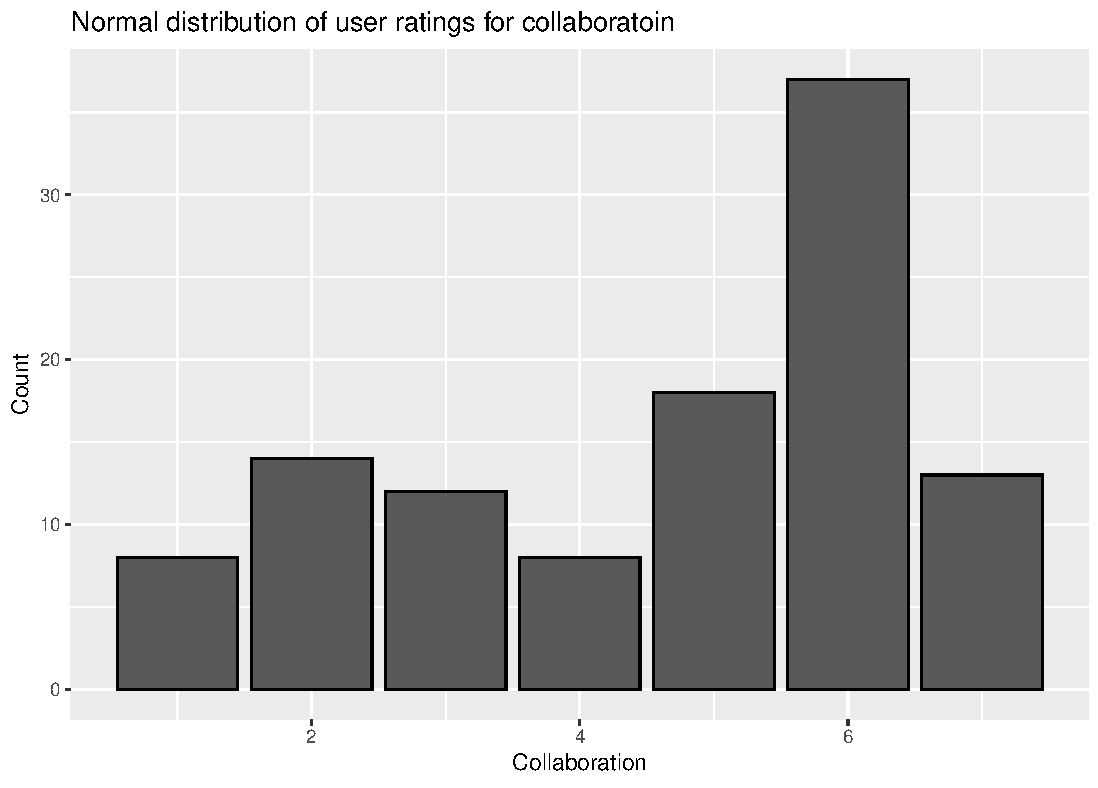
\includegraphics[width=0.8\linewidth]{Images/Graphs/H1CollabBar.pdf}
  
\caption{Bar chart displaying the distribution of collaboration ratings across both companions}
\label{fig:AppendixH1CollabBar}
\end{figure}

\clearpage

\subsection{Appendix - Testing Addendum}
\label{AppendixTesting}

\subsubsection{Appendix - Quality Assurance Plan}
\label{AppendixQAPlan}
%(Perry 1987)
%Correctness, Reliability, Efficiency, Integrity, Usability, Maintainability, Testability, Flexibility, Portability, Interoperability

%Types of Testing: Unit Testing, Automation and Continuous Integration, Run-Time Analyses, End-User Testing

The artefact will be tested in multiple stages. First, the basic combat mechanics and enemy AI will be playtested with end-users, which would most likely be friends and family, to ensure that there are no bugs that could interfere with the results of the experiment. I will gather vocal feedback and track any issues on a Trello board, which will be used to mark progress.

This is an important aspect as the basic mechanics will determine how the player interacts with the game and the decision-making for the companion agent relies on this.

When the basic combat mechanics and enemy AI are tested, the adaptive agent will go into testing. Unit tests will be used to confirm the calculations for generating the player model are correct and that the correct behaviours are chosen for the adaptive agent.

Once the adaptive agent has passed the unit testing, run-time testing will be used for optimisation. The aim is for the game to run at a minimum of 30 fps on the machines in the Games Academy. If the game isn't performant enough, the profiler in Unity will be used to find bottlenecks and fix them.

Before conducting the experiment, the game will be tested again with friends and family to ensure that the adaptive agent is behaving properly and to regulate difficulty. While game balance is not a primary concern here, the game should be challenging enough so that the companion provides clear use for the player, but is not overwhelming to distract the player from noticing them.

Throughout this process, regular builds will be made and tested to ensure that it works. Automated build generation may be used to make this process quicker.

Additionally, generating reference codes will need to be tested to ensure that multiple participants will not be given the same code. The initial plan for constructing the reference code is to construct multiple sets of digits. The first set of digits could be the current time, the next set could be randomly generated and the final digits could be determined by which AI the participant was given first. This system will need to be tested properly when it is developed.


\subsubsection{Appendix - Testing Evidence}
\label{AppendixUnitTests}

Figures \ref{fig:AppendixUnitEditTests} \ref{fig:AppendixUnitPlayTests} show the unit tests.

\begin{figure}[!h]
  \centering
  \includegraphics[width=0.75\linewidth]{Images/Unit Tests/EditTests.png}
  
\caption{Screenshot of the unit edit tests}
\label{fig:AppendixUnitEditTests}
\end{figure}

\begin{figure}[!h]
  \centering
  \includegraphics[width=0.6\linewidth]{Images/Unit Tests/PlayTests.png}
  
\caption{Screenshot of the unit play tests}
\label{fig:AppendixUnitPlayTests}
\end{figure}

\clearpage

Figure \ref{fig:AppendixIntegrationTest} shows a screenshot with the old user interface that displays the player state. This was used to test the player state was tested properly. Figure \ref{fig:AppendixRuntimeAnalysis} shows the frame-rate during gameplay.

\begin{figure}[!h]
  \centering
  \includegraphics[width=0.75\linewidth]{Images/Player State.png}
  
\caption{Screenshot of the game with the old UI showing player state}
\label{fig:AppendixIntegrationTest}
\end{figure}

\begin{figure}[!h]
  \centering
  \includegraphics[width=0.75\linewidth]{Images/Runtime Analysis.png}.
  
\caption{Screenshot of the game with the stats}
\label{fig:AppendixRuntimeAnalysis}
\end{figure}

\clearpage

\subsection{Appendix - Artefact Addendum}
\label{AppendixArtefact}

\subsubsection{Appendix - Links}
\label{AppendixLinks}

This section contains links to the repo and questionnaire forms

\textbf{Github Repository}:

\url{https://github.falmouth.ac.uk/Games-Academy-Student-Work-22-23/Buddy-NPC-Dissertation}

\textbf{Github Repository (Initial Prototype)}:

\url{https://github.falmouth.ac.uk/Games-Academy-Student-Work-22-23/Buddy-NPC-Dissertation/commit/493e0063025132e950696b4d174af48a5b190060}

\textbf{Github Repository (First Refactor)}:

\url{https://github.falmouth.ac.uk/Games-Academy-Student-Work-22-23/Buddy-NPC-Dissertation/commit/ff3c28e4a07d2bb3549c6dbc93962801a3e29a72}

\textbf{Microsoft Forms Questionnaire}:

\url{https://forms.office.com/Pages/ShareFormPage.aspx?id=s-4LVT1qRkahEfidAXd5LhYJGdgYND9Nn38bE3C1BhpUQVNUUkdQREdNWjQzV1BCRjE5MUUyOEZCTy4u&sharetoken=TNyfcCNSzhBCKWwSOgEt}

\textbf{Results Summary}:

\url{https://forms.office.com/Pages/AnalysisPage.aspx?AnalyzerToken=1N9wyxIbVfSuwC5N0kkWSdR5LMzd69cE&id=s-4LVT1qRkahEfidAXd5LhYJGdgYND9Nn38bE3C1BhpUQVNUUkdQREdNWjQzV1BCRjE5MUUyOEZCTy4u}

\subsubsection{Appendix - Trello Board}
\label{AppendixTrelloBoard}

Figure \ref{fig:AppendixTrelloBoard} shows the Trello board at the end of the development.

\begin{figure}[!h]
  \centering
  \includegraphics[width=\linewidth]{Images/TrelloBoard.png}
  
\caption{Screenshot of the Trello board}
\label{fig:AppendixTrelloBoard}
\end{figure}

\clearpage

\subsubsection{Appendix - UML Diagrams}
\label{AppendixUML}

Figures \ref{fig:AppendixCaseUML} \ref{fig:AppendixActivityUML} show the UML diagram of the AM companion agent.

\begin{figure}[!h]
  \centering
  \includegraphics[width=\linewidth]{Images/UML Diagrams/Case Diagram.pdf}
  
\caption{AM Agent Case Diagram}
\label{fig:AppendixCaseUML}
\end{figure}

\begin{figure}[!h]
  \centering
  \includegraphics[width=\linewidth]{Images/UML Diagrams/Activity diagram.pdf}
  
\caption{AM Agent Activity Diagram}
\label{fig:AppendixActivityUML}
\end{figure}

\clearpage


\subsection{Appendix - Ethics Addendum}
\label{AppendixEthics}

\subsubsection{Appendix - Participant Information and Consent Forms}
\label{AppendixEthicsForms}

Figure \ref{fig:AppendixInfoForm} shows the information sheet and figure \ref{fig:AppendixConsentForm} shows the consent form.

\begin{figure}[!h]
  \centering
  \includegraphics[width=0.8\linewidth]{Images/Ethics/Participant Information Form.pdf}
  
\caption{Image of the participant information sheet}
\label{fig:AppendixInfoForm}
\end{figure}

\begin{figure}[!h]
  \centering
  \includegraphics[width=0.8\linewidth]{Images/Ethics/Consent Form.pdf}
  
\caption{Image of the consent form}
\label{fig:AppendixConsentForm}
\end{figure}

\clearpage

\subsubsection{Appendix - Risk Assessment}
\label{AppendixRiskAssessment}

Figure \ref{fig:AppendixRiskAssessment} shows images of the risk assessment and risk matrix.

\begin{figure}[!h]
  \centering
  \includegraphics[width=0.70\linewidth]{Images/Ethics/Risk Assessment(1).png}
  \includegraphics[width=0.70\linewidth]{Images/Ethics/Risk Assessment(2).png}
  
\caption{Image of the risk assessment and risk matrix}
\label{fig:AppendixRiskAssessment}
\end{figure}

\clearpage

\end{document}